\subsubsection{Social features}
\label{sec:methods_features_social}

So far, there were explained traditional financial features, then Bitcoin and
bitcoin features, and finally structural break features to introduce SADF
computation. Nevertheless, nothing has been said about the agents that operate
in this market so far. Therefore, what follows shows some figures to illustrate
the data gathered from the two sources: Google Trends and
Alternative.me.

First, in figure \ref{fig:google_trends} the bitcoin price series is shown
together with the interest index that Google Trends offers. Note that a linear
interpolation was used to fit daily values because social data was available
only a weekly basis. We can see that there is a better fit between the curve
shapes in the third regime and after the third halving on.

Finally, in figure \ref{fig:alternative_me} the sentiment index is displayed
for the last two periods. Data for the first two two periods was not available.
It is worth mentioning that this series is the result of fused data from
Twitter, Reddit and other forums which is definitely richer than Google Trends
interest index. Google Trends is just used to compensate social information
during the first two periods.

\begin{figure}[H]
    \centering
    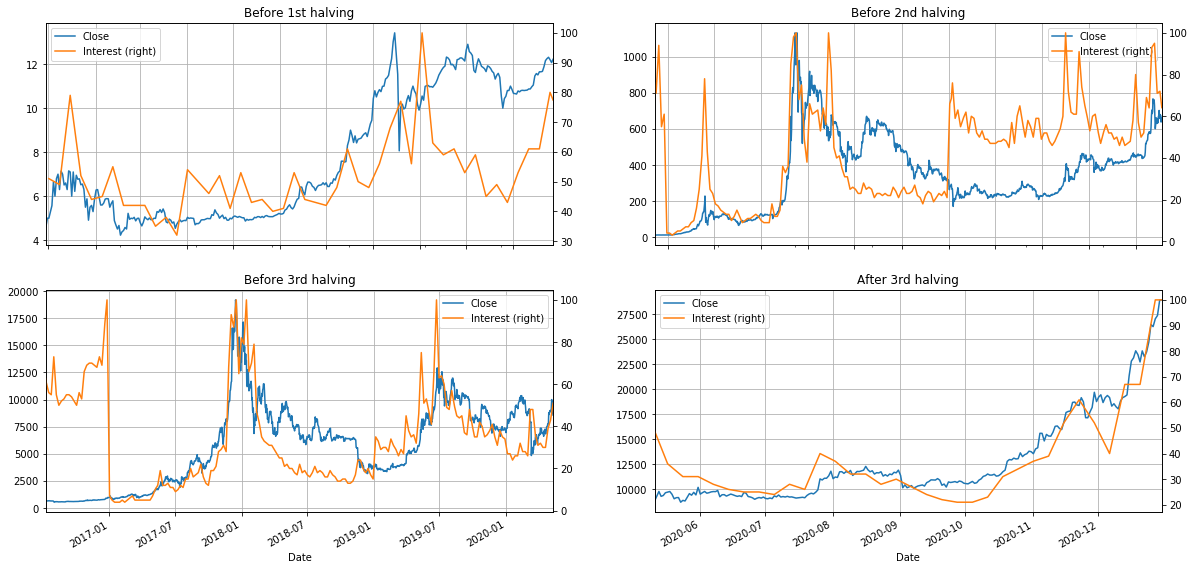
\includegraphics[width=\textwidth]{methods/images/gtrends_price_per_halving.png}
    \caption{Evolution over each bitcoin regime of the Google Trends interest in the "bitcoin" keyword together with the close price of bitcoin.}
    \label{fig:google_trends}
\end{figure}

\begin{figure}[H]
    \centering
    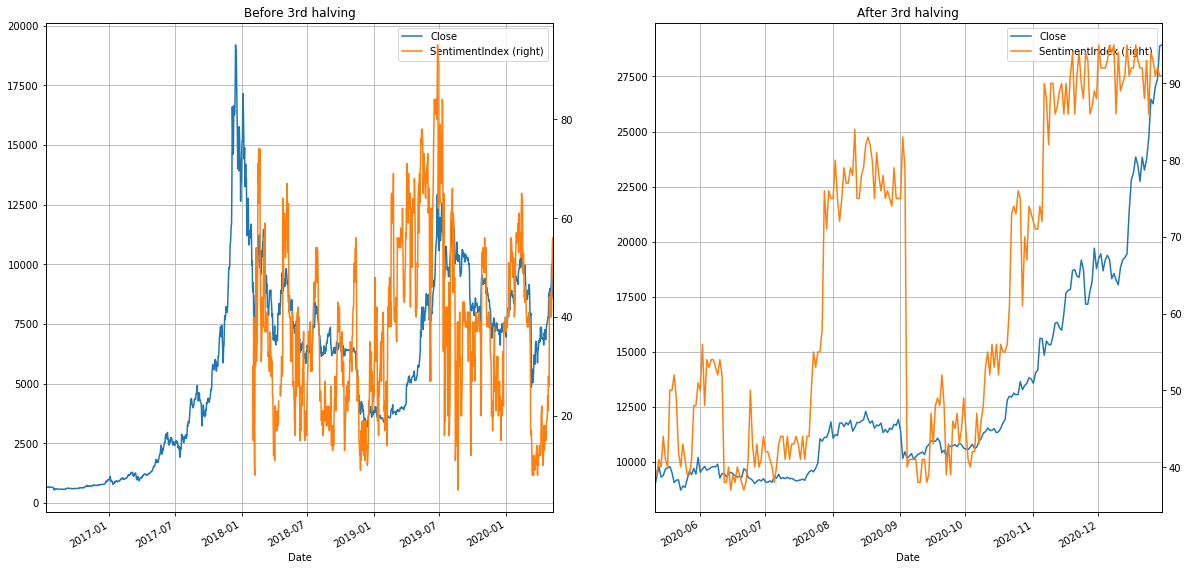
\includegraphics[width=\textwidth]{methods/images/alternative_me_halvings.png}
    \caption{Evolution over the last two bitcoin's regimes of the Alternative.me social interest of bitcoin together with the close price of bitcoin.}
    \label{fig:alternative_me}
\end{figure} 